\documentclass[11pt]{article}
\usepackage[margin=1in]{geometry}
\usepackage[T1]{fontenc}
\usepackage[utf8]{inputenc}
\usepackage{lmodern,microtype}
\usepackage{amsmath,amssymb,amsthm,mathtools}
\usepackage{graphicx,booktabs,array,enumitem,setspace,placeins}
\usepackage{algorithm}
\usepackage{algpseudocode}
\usepackage{needspace}
\usepackage[authoryear,round]{natbib}
\usepackage{xr-hyper}
\usepackage[colorlinks=true,allcolors=blue]{hyperref}
\usepackage{bookmark}
\allowdisplaybreaks
\setstretch{1.18}
\setlength{\parskip}{0pt}
\setlength{\emergencystretch}{2em}
\setlist{itemsep=2pt,topsep=4pt}
\newtheorem{theorem}{Theorem}[section]
\newtheorem{lemma}[theorem]{Lemma}
\newtheorem{proposition}[theorem]{Proposition}
\newtheorem{corollary}[theorem]{Corollary}
\newtheorem{definition}[theorem]{Definition}
\newtheorem{example}[theorem]{Example}
\theoremstyle{remark}
\newtheorem{remark}[theorem]{Remark}
\newcommand{\E}{\mathbb E}
\newcommand{\Prob}{\mathbb P}
\newcommand{\ind}{\mathbf 1}
\newcommand{\kl}{\operatorname{kl}}
\newcommand{\pos}[1]{\left[#1\right]_+}
\newcommand{\suppproof}{Complete proofs appear in the supplementary material.}

\externaldocument[][nocite]{revision_2026-10-16/build/supplement}[supplement.pdf]
% Set \anonymoustrue for an author-free review copy if required by the portal.
\newif\ifanonymous
\anonymousfalse
\title{The Cost of Reliable Near-Optimal Set Maintenance\\with Arriving Arms}
\ifanonymous
\author{}
\else
\author{Deqi Zheng\thanks{The first two authors contributed equally.} \quad
 Xiaoyang Xu\footnotemark[1] \\ Qiuzhen College, Tsinghua University
 \and Yuhong Yang\thanks{Corresponding author: yyangsc@mail.tsinghua.edu.cn.}\\
 Yau Mathematical Sciences Center, Tsinghua University}
\fi
\date{October 15, 2026}
\ifanonymous
\hypersetup{pdftitle={The Cost of Reliable Near-Optimal Set Maintenance with Arriving Arms},pdfauthor={}}
\else
\hypersetup{pdftitle={The Cost of Reliable Near-Optimal Set Maintenance with Arriving Arms},pdfauthor={Deqi Zheng, Xiaoyang Xu, Yuhong Yang}}
\fi
\begin{document}
\maketitle

\begin{abstract}
We study the cost of maintaining reliable reports of all relatively
near-optimal arms while collecting rewards when new arms arrive and remain
available. Reward laws are stationary, but each arrival can change the
membership boundary. We measure reporting progress by cumulative unresolved
arm time outside a prescribed boundary band, under simultaneous correctness
of all issued labels. Uncertainty about one new arm can obstruct positive
certification of many earlier candidates. A lower bound in one common
reference environment quantifies this effect. We obtain matching
worst-schedule orders for unresolved area and an arrival-growth boundary
for jointly sublinear area and expected regret. On a specified
repeated-update family, rapid maintenance requires inverse-square regret,
whereas a constant-factor larger area budget admits a logarithmic regret
upper bound. The rapid cost also holds with nonvanishing probability in a
fixed environment. A fixed-precision checkpoint construction provides the
upper bounds without knowing future arrivals. Finite-budget comparisons
show that its conservative certification cost can be substantial; they
do not establish uniform numerical superiority or a general optimal
regret--area frontier.
\end{abstract}
\noindent\textit{Keywords:} sequential experimentation; arriving arms;
near-optimal set maintenance; dynamic regret; simultaneous inference.

\section{Introduction}
\label{sec:introduction}

Sequential experiments often acquire new candidates while earlier ones remain
available. An allocation rule must learn which candidates yield high rewards.
An experimenter may also need to know which of all available candidates are
within a specified tolerance of the current best. These objectives need not
favor the same observations. A candidate can be sufficiently inferior to
receive little reward-driven exploration and still be difficult to classify
relative to the near-optimality boundary.

We study these objectives together under permanent exogenous arrivals and
stationary reward laws. If $r^*(t)$ is the largest mean among the arms
available at time $t$, an arm is relatively near-optimal when its mean is at
least $r^*(t)-\varepsilon$. Reports certify membership, certify exclusion, or
leave the arm unresolved. We require one simultaneous correctness event for
all labels at all times. To rule out indefinite abstention, we charge the
cumulative unresolved time of arms whose means lie more than $\eta$ from
the membership boundary. The question is how much regret is necessary, and
how much is attainable, under this reporting requirement.

New arrivals affect the task in two ways. An uncertain new candidate may be
better than the incumbent by enough to invalidate many existing positive
reports. Evidence about that one candidate is then relevant to many
reports at once. A later improvement can also make an earlier difficult
membership question unnecessary: a candidate close to the old boundary may
be far below the new one. Its existing upper confidence bound can be
combined with a new reference's lower bound to certify exclusion. Neither
effect requires the reward law of an old arm to change.

Our observation model and regret comparator have established precedents.
Permanent arrivals form a monotone special case of sleeping-bandit
availability \citep{kleinberg2010}; ballooning bandits already compare reward
with the best arm currently available \citep{ghalme2021}. Exogenous arrivals
differ from drawing arms on demand from a reservoir
\citep{10.1214/aos/1069362389} and from the disappearing actions of mortal
bandits \citep{NIPS2008_788d9869}. Benchmark improvements here arise from new
arms, whereas nonstationary bandits allow the reward distributions of
existing arms to change \citep{Besbes2014,Auer2019ADSWITCH}. Sequential
allocation and adaptive experimentation have a long statistical history
\citep{Robbins1952,LAI19854,Lai1987}; the expanding set of actions retains
that allocation problem and adds an evolving inferential target.

For a fixed arm set, identifying every relatively near-optimal arm is the
ALL-$\varepsilon$ problem \citep{mason2020}. Joint reward and identification
objectives also have established precedents
\citep{degenne2019,yang2026,cho2025}. Our task requires continuing reports
under arrivals, with all-time label reliability and an explicit cumulative
cost for unresolved arm time. The distinction concerns the reporting
protocol and its cost, rather than a new arriving-arm model. The simultaneous
recovery scales used in our lower bounds build on existing information
inequalities and multiple-recovery arguments
\citep{kaufmann2016,malloy2014,jamieson2018}.

We give three results about maintenance cost. First, a common-reference
lower bound shows how one uncertain arrival can obstruct many other
certifications. Its information queue accumulates cost over time within
one reward environment. Second, we obtain matching worst-schedule orders
for cumulative unresolved area, including finite-horizon truncation, and
derive the polynomial arrival boundary for jointly sublinear area and
expected regret. This worst-case lower bound already occurs in an initial
static batch; the common-reference result describes a separate consequence
of continuing arrivals. Third, on a specified repeated-update family,
rapid resolution of temporary membership tasks has matching inverse-square
regret costs. Allowing a constant-factor larger area budget admits a
logarithmic regret upper bound. A nonvanishing-probability lower bound
holds in one fixed environment under the same cumulative-area requirement.
The deferred endpoint has only an upper bound, and the general frontier
over intermediate budgets and overlapping arrivals remains open.

An explicit fixed-precision procedure, Checkpoint-UCB, supplies the
attainability results. It shares all observations between certification
and reward learning and retains every arrived arm in reward selection.
The construction separates the statistical costs cleanly, but its
conservative quotas can exceed a practical budget. Our numerical study
retains those failures as well as favorable comparisons. Section~\ref{sec:model}
defines the joint task, Section~\ref{sec:method} gives the construction,
and Sections~\ref{sec:maintenance}--\ref{sec:tradeoff} establish the
maintenance and regret bounds. Section~\ref{sec:experiments} examines their
finite-budget implications.

\section{Model, reliable reports, and maintenance cost}
\label{sec:model}
\label{sec:problem}

\subsection{Observation model and regret}

Let $\mathcal A$ be a possibly infinite set of arms. Arm $i$ arrives at
time $\tau_i$, after which it remains available. At every physical time
$t=1,2,\ldots$,
\[
 \mathcal A_t=\{i:\tau_i\le t\},\qquad
 1\le K_t=|\mathcal A_t|<\infty.
\]
Arbitrary finite batches are allowed, including $K_T>T$ at an evaluation
endpoint. Each arm has an unknown stationary reward law on $[0,1]$ with
mean $r_i$. Its successive potential observations $(Y_{i,n})_{n\ge1}$ are
independent and identically distributed, and the streams of different arms
are independent. Arrivals are exogenous and independent of both these
streams and policy randomization. Unless stated otherwise, each result
is for a fixed deterministic arrival schedule.

At time $t$, the policy first receives all current arrivals, then selects
one arm $I_t\in\mathcal A_t$, observes one reward $X_{t,I_t}$, and finally
issues its report. It uses the observed history
\[
 H_{t-1}=(\mathcal A_s,I_s,X_{s,I_s})_{s=1}^{t-1}
\]
and independent randomization. Means, future arrivals, and true membership
labels are unavailable to the policy. With
$N_i(t)=\sum_{s\le t}\ind\{I_s=i\}$, the physical observation is
$X_{t,I_t}=Y_{I_t,N_{I_t}(t-1)+1}$. Write
\[
 \hat r_i(n)=\frac1n\sum_{s=1}^nY_{i,s},\qquad
 r^*(t)=\max_{i\in\mathcal A_t}r_i,\qquad
 \Delta_i(t)=r^*(t)-r_i \quad(i\in\mathcal A_t).
\]
At a deterministic endpoint $T$, cumulative dynamic regret is
\[
 R_T(\pi)=\sum_{t=1}^{T}\Delta_{I_t}(t).
\]
This is a sum of mean gaps, random through the policy's arm selections;
$\E R_T$ is its expectation. The quantity does not compare realized
reward sequences. Physical time always counts actual observations.

\subsection{Reliable reports and cumulative unresolved time}
\label{sec:reporting_task}

For $0<\varepsilon<1$, the target set is
\[
 \mathcal G_t^\varepsilon=\{i\in\mathcal A_t:\Delta_i(t)\le\varepsilon\}.
\]
After the current observation, a report partitions all of $\mathcal A_t$
into $\mathcal P_t,\mathcal N_t,\mathcal V_t$: certified members, certified
nonmembers, and unresolved arms. Define
\[
 E_{\rm lab}=\{\text{for all }t:\ \mathcal P_t\subseteq\mathcal G_t^\varepsilon
                  \subseteq\mathcal A_t\setminus\mathcal N_t\}.
\]
A policy is $\delta$-reliable if $\Prob(E_{\rm lab})\ge1-\delta$ in every
allowed reward environment. A positive report may be withdrawn after a new
arrival. On the correctness event, a negative report remains valid because
$r^*(t)$ is nondecreasing and the arm's mean is stationary.

Reliability permits all arms to remain unresolved. For a boundary width
$0<\eta<1$, define
\begin{equation}
 \begin{split}
 d_i^\varepsilon(t)&=|\Delta_i(t)-\varepsilon|,\\
 U_t(\eta)&=\sum_{i\in\mathcal A_t}
   \ind\{i\in\mathcal V_t,d_i^\varepsilon(t)>\eta\},\qquad
 \mathcal U_T(\eta)=\sum_{t=1}^{T}U_t(\eta).
 \end{split}
 \label{eq:area}
\end{equation}
The count includes newly arrived arms with no observations and old arms
that become unresolved again. Every such arm--time pair is charged; the
loss is not limited to the time before a first decision. Within the
boundary band, unresolved time is exempt, but any label issued there must
still be correct. The true distance $d_i^\varepsilon(t)$ is used only by
the evaluator and in the analysis.

The task parameters are fixed when comparing policies. Their roles are
summarized below.
\begin{center}
\begin{tabular}{cl}
\toprule
Parameter & Meaning\\
\midrule
$\varepsilon\in(0,1)$ & Relative near-optimality tolerance\\
$\delta\in(0,1/2)$ & Joint error budget\\
$\eta\in(0,1)$ & Boundary width exempting unresolved time\\
$\rho\in(0,1)$ & Predetermined precision of reporting checkpoints\\
\bottomrule
\end{tabular}
\end{center}

The main requirement at a fixed $T$ is
\begin{equation}
 \E_\theta R_T\le r,\qquad
 \Prob_\theta\{E_{\rm lab},\mathcal U_T(\eta)\le a\}\ge1-\delta.
 \label{eq:joint_protocol}
\end{equation}
It combines an expected regret bound with a joint high-probability
label--area guarantee. In particular, $\mathcal U_T=o(T)$ requires the
time-average number of unresolved separated arms to vanish, rather than
only a small unresolved fraction of all arms. The area guarantee is for
each deterministic endpoint; it need not hold for every endpoint on one
common area event.

For a performance family $\Theta$, let $\mathfrak R_\Theta(a)$ be the
infimum of $\sup_{\theta\in\Theta}\E_\theta R_T$ over policies reliable on
the full bounded model and satisfying the probability condition in
\eqref{eq:joint_protocol} for every $\theta\in\Theta$. The value is
$+\infty$ if the feasible class is empty. Full-model label reliability
and a family-specific area guarantee are distinct requirements. The
lower bounds remain valid when reliability is required only on the
lower-bound subfamily.

\subsection{How arrivals change the reporting problem}

For a fixed old arm, $\Delta_i(t)$ is nondecreasing, so its true membership
can change only from member to nonmember. Its boundary distance
$|\Delta_i(t)-\varepsilon|$ need not be monotone. A new candidate can first
create uncertainty about the current best mean, obstructing positive
certification of many old arms even when those arms remain truly
near-optimal. A sufficiently good new reference can later move the
boundary past earlier candidates, making their fine classification
unnecessary. Sections~\ref{sec:maintenance} and~\ref{sec:tradeoff} quantify
these two effects under the same reporting protocol.

\section{A checkpoint construction for joint guarantees}
\label{sec:method}

The upper bounds use a fixed-precision construction, Checkpoint-UCB. Its
reporting intervals are formed once, while its reward estimates use every
observation. Index arms by arrival order $i=1,2,\ldots$, with a fixed order
within each batch. Choose $0<\rho<1$ before observing rewards and set
\begin{equation}
 q_i(\rho)=\left\lceil\frac2{\rho^2}
                  \log\frac{4i(i+1)}\delta\right\rceil.
 \label{eq:checkpoint}
\end{equation}
Before this lifetime count is reached, arm $i$ has reporting interval $[0,1]$.
At its $q_i$th observation the interval becomes permanently
\begin{equation}
 [\ell_i,u_i]=[\hat r_i(q_i)-\rho/2,
                 \hat r_i(q_i)+\rho/2]\cap[0,1].
 \label{eq:fixed_interval}
\end{equation}
Although its completion time is adaptive, the
interval uses a predetermined potential prefix. Different precisions
$\rho_i$ may also be prescribed before the corresponding arms are observed;
data-dependent checkpoint selection is not covered.

At even times the policy serves the first incomplete checkpoint in arrival
order, if one remains. At every other time it maximizes, over all
$i\in\mathcal A_t$,
\begin{equation}
 J_i(t)=\hat r_i(N_i(t-1))+
             \sqrt{\frac{3\log(2t)}{N_i(t-1)}}.
 \label{eq:ucb}
\end{equation}
A zero count gives index $+\infty$; ties are broken by the smallest
arrival-order label. Both kinds of pull update the same count and reward
sum. After observing the selected reward, define
$\underline r^*(t)=\max_{i\in\mathcal A_t}\ell_i$ and
$\overline r^*(t)=\max_{i\in\mathcal A_t}u_i$, and report
\begin{equation}
 \mathcal P_t=\{i:\ell_i\ge\overline r^*(t)-\varepsilon\},\qquad
 \mathcal N_t=\{i:u_i<\underline r^*(t)-\varepsilon\},\qquad
 \mathcal V_t=\mathcal A_t\setminus(\mathcal P_t\cup\mathcal N_t).
 \label{eq:reports}
\end{equation}

\begin{algorithm}[p]
\caption{Checkpoint-UCB}
\label{alg:checkpoint-ucb}
\begin{algorithmic}[1]
\Require $\varepsilon\in(0,1)$, $\delta\in(0,1/2)$, predetermined $\rho\in(0,1)$
\State $\mathcal A^{\rm cur}\gets\varnothing$, FIFO queue $\mathcal Q^{\rm srv}\gets\varnothing$, $k\gets0$
\For{physical time $t=1,2,\ldots$}
  \For{each arm arriving at $t$, in a fixed within-batch order}
    \State $k\gets k+1$; assign label $i\gets k$; $\mathcal A^{\rm cur}\gets\mathcal A^{\rm cur}\cup\{i\}$
    \State $n_i\gets0$, $s_i\gets0$, $[\ell_i,u_i]\gets[0,1]$
    \State $q_i\gets\left\lceil(2/\rho^2)\log\{4i(i+1)/\delta\}\right\rceil$; append $i$ to $\mathcal Q^{\rm srv}$
  \EndFor
  \While{$\mathcal Q^{\rm srv}\ne\varnothing$ and $n_{\operatorname{front}(\mathcal Q^{\rm srv})}\ge q_{\operatorname{front}(\mathcal Q^{\rm srv})}$}
    \State Remove the front of $\mathcal Q^{\rm srv}$
  \EndWhile
  \If{$t$ is even and $\mathcal Q^{\rm srv}\ne\varnothing$}
    \State $I\gets\operatorname{front}(\mathcal Q^{\rm srv})$ \Comment{designated service pull}
  \Else
    \State $J_i\gets+\infty$ if $n_i=0$, and $J_i\gets s_i/n_i+\sqrt{3\log(2t)/n_i}$ otherwise, for $i\in\mathcal A^{\rm cur}$
    \State $I\gets\min\operatorname*{arg\,max}_{i\in\mathcal A^{\rm cur}}J_i$
  \EndIf
  \State Pull $I$ once and observe $x$; $n_I\gets n_I+1$, $s_I\gets s_I+x$
  \If{$n_I=q_I$}
    \State $m\gets s_I/q_I$; $\ell_I\gets\max\{0,m-\rho/2\}$, $u_I\gets\min\{1,m+\rho/2\}$
  \EndIf
  \State $L\gets\max_{i\in\mathcal A^{\rm cur}}\ell_i$, $U\gets\max_{i\in\mathcal A^{\rm cur}}u_i$
  \State $\mathcal P_t\gets\{i\in\mathcal A^{\rm cur}:\ell_i\ge U-\varepsilon\}$, $\mathcal N_t\gets\{i\in\mathcal A^{\rm cur}:u_i<L-\varepsilon\}$
  \State $\mathcal V_t\gets\mathcal A^{\rm cur}\setminus(\mathcal P_t\cup\mathcal N_t)$; report $(\mathcal P_t,\mathcal N_t,\mathcal V_t)$
\EndFor
\end{algorithmic}
\end{algorithm}

Algorithm~\ref{alg:checkpoint-ucb} observes exactly one reward per physical
round. Its variables $n_i$ and $s_i$ are the lifetime count and reward sum.
An ordinary UCB pull can complete any checkpoint, including one behind the
queue's front. The queue discards such completed entries when they reach its
front. An interval is computed only when $n_i=q_i$, and is not recomputed
when $n_i>q_i$. Reaching $q_i$ forms fixed-precision evidence; it need not
produce a determinate report if other arms are still uncertain or the arm
lies closer to the boundary than that evidence can resolve.

All arrived arms remain eligible for \eqref{eq:ucb}, including negatively
reported arms. The intervals are nonempty on every path, so
$\mathcal P_t$ and $\mathcal N_t$ are disjoint. A count, sum, and interval
are stored for every arm; a direct index or report update costs $O(K_t)$
operations. The policy uses no terminal horizon, future arrivals, true means,
or reference identities.

\begin{proposition}[Simultaneous reporting and unconditional reward cost]
\label{prop:reporting}
On the full bounded model, Checkpoint-UCB satisfies
$\Prob(E_{\rm lab})\ge1-\delta/2$. If $\mathcal I_T$ is its set of designated
service time steps, then at every deterministic $T$,
\begin{equation}
 \E R_T\le\min\left\{T,K_T+4\sqrt{3K_TT\log(2T)}+1+
                \E\sum_{t\in\mathcal I_T}\Delta_{I_t}(t)\right\}.
 \label{eq:reward_bound}
\end{equation}
Pathwise, $|\mathcal I_T|\le\sum_{i\le K_T}q_i$.
\end{proposition}

Hoeffding's inequality bounds the failure at checkpoint $i$ by
$\delta/\{2i(i+1)\}$. Summing over potential arm indices gives one coverage
event of probability at least $1-\delta/2$, on which every report is correct.
For \eqref{eq:reward_bound}, a separate, summable concentration argument at
physical time $t$ controls ordinary UCB pulls. Each arm and pre-pull count
is charged at most once; inserted service observations only skip counts.
This expectation bound holds without conditioning on reporting success,
so it omits no $\delta T$ term. It bounds one policy's total regret, rather
than a regret difference between its trajectory and a hypothetical policy
without service. \suppproof

\section{Fundamental costs of continual maintenance}
\label{sec:maintenance}

\subsection{One uncertain arrival can obstruct many reports}

The first lower bound retains one reward environment throughout the time axis.
It therefore measures a cumulative burden without adding the worst cases of
incompatible experiments. Fix
$0<\varepsilon\le1/16$, $0<\delta\le1/16$, and $0<\eta<\varepsilon/2$.
An initial reference has Bernoulli mean $1/4+\varepsilon/2$. Candidates arrive
on any prescribed schedule. In environment zero each has mean $p=1/4$;
environment $j$ changes only candidate $j$ to mean $p+2\varepsilon$.
All candidates are good in environment zero, with boundary distance
$\varepsilon/2$. After candidate $j$ arrives in environment $j$, every other
candidate is bad.

Let $M_t$ count arrived candidates and $a_t=M_t-M_{t-1}$. Define
\begin{align}
 q_-&=\left\lfloor\frac{\kl(1/4,\delta)}
                              {\kl(1/4,1/4+2\varepsilon)}\right\rfloor,
 &Q_t&=(Q_{t-1}+q_-a_t-1)_+,\quad Q_0=0,\notag\\
 \mathcal B_T&=\sum_{t\le T}(M_t-1)_+\ind\{Q_t>0\}.
 \label{eq:broadcast_queue}
\end{align}
This analytical queue is an information-capacity certificate: arrivals add
$q_-$ units per candidate, while only one observation is possible per round.
It is distinct from the algorithm's FIFO queue $\mathcal Q^{\rm srv}$ and
does not impose a pathwise sampling quota on every candidate. In the stated
range $q_-\ge2$.

\begin{theorem}[Broadcast uncertainty]
\label{thm:broadcast}
For every policy reliable on environment zero and all its one-candidate
alternatives,
\[
 \E_0\mathcal U_T(\eta)\ge(3/4-\delta)\mathcal B_T.
\]
If $\mathcal B_T>0$, then
\[
 \Prob_0\{\mathcal U_T(\eta)\ge\mathcal B_T/4\}\ge1/4.
\]
These conclusions still hold when the policy knows the full arrival schedule,
the horizon, and the reference distribution.
\end{theorem}

At a busy time, some deterministic candidate label has expected sample count
below $q_-$. Changing that candidate alone has too little history KL to permit
positive certification of another candidate with probability at least $1/4$.
Reliability also bounds incorrect negative reports. The remaining probability
must be unresolved. The same reference environment supports this argument at
every time; the difficult label is selected from expected counts rather than
from a favorable realized history. The supplementary proof includes the
bounded-variable step needed for the probability statement.

If $m$ candidates have arrived by time $s$, the queue obeys the deterministic
inequality
\begin{equation}
 \sum_{t\le s+qm-1}(M_t-1)_+\ind\{Q_t(q)>0\}
                  \ge\frac{q-1}{2}m(m-1),\qquad q\ge2.
 \label{eq:queue_area}
\end{equation}
The factor $m^2$ reflects the number of affected reports as well as the work
needed to exclude high-quality alternatives. The subtraction of one unit in
$q-1$ accounts for the last observation of each busy period: reports are issued
after service.

\subsection{Worst-schedule maintenance area}

Let $\mathfrak A_{T,K}$ be the smallest $a$ attainable by a full-model reliable
policy with
\[
 \sup_{\boldsymbol\tau:K_T\le K}\sup_{\boldsymbol r}
 \Prob_{\boldsymbol r}\{E_{\rm lab}^c\ \text{or}\ \mathcal U_T(\eta)>a\}\le\delta.
\]
This optimization imposes no regret budget. Policies may know $T,K$ and the
schedule for the lower bound. The upper bound uses neither $T$ nor $K$ as
input.

\begin{theorem}[Worst-schedule area and joint attainability]
\label{thm:worst_area}
For integers $K\ge2$ and $T\ge1$, $0<\varepsilon\le1/8$,
$0<\eta\le\varepsilon/32$, and $0<\delta\le1/16$,
\begin{equation}
 2^{-24}\min\left\{KT,\frac{K^2}{\eta^2}\log\frac K\delta\right\}
 \le\mathfrak A_{T,K}\le
 256\min\left\{KT,\frac{K^2}{\eta^2}\log\frac K\delta\right\}.
 \label{eq:worst_area}
\end{equation}
Checkpoint-UCB with $\rho=\eta/4$ attains the upper order and also satisfies
\begin{equation}
 \E R_T\le\min\left\{T,K+4\sqrt{3KT\log(2T)}+1+
                         99K\eta^{-2}\log(K/\delta)\right\}.
 \label{eq:joint_general}
\end{equation}
\end{theorem}

For the upper bound, completed checkpoints imply endpoint errors at most
$\eta/4$, sufficient to classify all arms outside the boundary band. The
unfinished-work queue is dominated by adding $q_i$ at each arrival and serving
at even rounds. On the simultaneous coverage event,
\begin{equation}
 \mathcal U_T(\eta)\le\min\left\{K_TT,
                         2K_T\sum_{i\le K_T}q_i\right\}.
 \label{eq:queue_upper}
\end{equation}
Additional UCB observations reduce the work; they are not charged again as
new checkpoint samples. The lower bound uses $K-1$ candidates with independent
means $1/2\pm2\eta$ and a reference of mean $1/2+\varepsilon$, all available
at the first pull. Simultaneous partial recovery and a horizon truncation give
the probability statement required by the definition of $\mathfrak A_{T,K}$.
The statistical $\log K$ factor has fixed-arm multiple-testing precedents;
this worst-schedule lower construction itself requires no repeated arrivals.

\subsection{Growth rates and the limits of total-count criteria}

\begin{corollary}[Arrival-growth boundary]
\label{cor:growth}
Fix the task parameters of Theorem~\ref{thm:broadcast} and one infinite arrival
schedule. If a policy is reliable for every reward environment and has a
deterministic envelope $a_T=o(T)$ satisfying \eqref{eq:joint_protocol} in
every environment, then $K_t=o(\sqrt t)$. Conversely,
$K_T^2\log(eK_T)=o(T)$ suffices for one horizon-free policy to have both
$\E R_T=o(T)$ and such a sublinear area envelope. In particular, for
$K_t\asymp t^\alpha$, $0<\alpha<1$, simultaneous attainment is possible if
and only if $\alpha<1/2$.
\end{corollary}

The necessity follows from \eqref{eq:queue_area}. For sufficiency, the general
checkpoint completion bound in Supplementary Lemma~\ref{app:completion_general}
applies throughout $0<\eta<\varepsilon/2$, together with
Proposition~\ref{prop:reporting}. This argument does not require the narrower
range $\eta\le\varepsilon/32$ in Theorem~\ref{thm:worst_area}. The exponent
statement leaves a logarithmic gap for general critical schedules.

Within the parameter range of Theorem~\ref{thm:worst_area},
\eqref{eq:worst_area} also gives a uniform terminal-count statement: over all
schedules with $K_T\le k(T)$, sublinear expected regret and sublinear service
envelopes are jointly attainable if and only if
$k(T)^2\log k(T)=o(T)$. Here the worst schedule can change with $T$.
This statement concerns a different schedule class from the single infinite
schedule in Corollary~\ref{cor:growth}.

The necessary condition $K_t=o(\sqrt t)$ is not sufficient on every fixed
schedule. For example, batches of size
\[
 m_n=\left\lfloor\frac{\sqrt{s_n}}{(\log s_n)^{1/4}}\right\rfloor,
 \qquad s_n=2^{2^n},
\]
give $K_t=o(\sqrt t)$ but preclude any $o(T)$ area envelope uniform over
reward environments. Near $s_n$, simultaneous classification of that burst
requires accumulated unresolved area of order $m_n^2\log m_n$, which exceeds
$s_n$ by a growing factor. The supplementary argument selects a single
infinite schedule; the difficult reward environment is allowed to vary with
the endpoint, as required by the stated uniform guarantee.

\section{Temporary membership tasks and regret trade-offs}
\label{sec:tradeoff}

\subsection{A repeated-update family}

We keep the reward environment, arrival schedule, endpoint, and reporting
parameters fixed when comparing two area budgets. Choose integers $J\ge1$,
$M\ge\max\{2,J\}$ and
\begin{equation}
 0<\varepsilon\le1/8,\quad 0<\delta\le1/16,\quad
 0<v,\quad Jv\le\varepsilon/4,\quad 0<d\le v/32,\quad\eta=d/2.
 \label{eq:family_parameters}
\end{equation}
At $a_e=1+eH$, $e=0,\ldots,J$, a reference with mean $b_e=1/2+ev$
arrives. For each $e<J$, the same batch contains $M$ candidates with means
\begin{equation}
 r_{e,k}=b_e-\varepsilon+\sigma_{e,k}d,
           \qquad \sigma_{e,k}\in\{-1,+1\}.
 \label{eq:family_means}
\end{equation}
All rewards are Bernoulli and all arms remain available. The last batch
contains only its reference, and $T=(J+1)H$. The family $\Theta$ includes
every sign configuration and every within-batch permutation. The policy is
not told which arm is the reference. Lower bounds may disclose those
identities and the schedule.

In its birth window a candidate is good exactly when its sign is positive.
Its reward gap is $\varepsilon-\sigma_{e,k}d$, while its distance to the
membership boundary is $d$. At the next update its gap becomes
$\varepsilon+v-\sigma_{e,k}d$, so both signs are bad, with boundary distance
at least $v-d$. Every reference remains good: the final good set consists of
all references. The tasks that distinguish the candidate signs expire even
though their arms remain available. The restriction $Jv\le\varepsilon/4$
limits the number of updates at any fixed positive improvement size.

\subsection{Low area forces enough temporary tasks to finish}

The lower-bound ingredient permits arbitrary interleaving and stopping. For
$m$ independent uniform signs with observation laws $P_i^+,P_i^-$, put
\[
 \kappa=\max_i\max\{D(P_i^+\Vert P_i^-),D(P_i^-\Vert P_i^+)\}
                                                    \in(0,\infty).
\]
If a bounded stopping time has at least half the signs determined with prior
probability at least $1/2$, and all configurations have familywise report
error at most $\delta\le1/16$, then
\begin{equation}
 \overline\E\sum_{i=1}^mN_i\ge
                 \frac{m}{1024\kappa}\log\frac m\delta.
 \label{eq:partial_recovery}
\end{equation}
Other observations must not encode these signs. The proof factors the
conditional posterior after the adaptive sampling and bounded stopping
kernels cancel, and combines simultaneous recovery with coordinatewise
change of measure \citep{kaufmann2016}. It does not assume independence of
the random sample counts. The product prior is a proof device; the final
lower bound concerns a fixed environment.

A window that never reaches half-completion contributes at least $MH/2$
area. Thus, on the event $\mathcal U_T(\eta)\le V/8$, where $V=JMH$, at
least $3J/4$ windows half-complete. A common product prior over all windows
turns this area requirement into enough instances of
\eqref{eq:partial_recovery}. Each candidate observation costs at least
$\varepsilon-d$ regret, and observations from distinct batches are charged
once. This argument does not impose a deadline on every individual batch;
the policy can choose where to defer. The heterogeneous completion
probabilities and their information-allocation relaxation are given in
Supplementary Section~\ref{app:area_lower}. That relaxation is a necessary
constraint, with no general causal attainability claim.

\subsection{Shared evidence for area and reward guarantees}

Checkpoint-UCB may use a predetermined precision $\rho_e$ for each arriving
batch. Consider the heterogeneous repeated-update family: batch $F_e$ has
reference mean $b_e$ and $M_e$ candidate means
$b_e-\varepsilon\pm d_e$, all in the allowed reward range. The windows
partition physical times $1,\ldots,T$; write $a_e$ for the arrival time of
batch $e$, $H_e$ for its window length, and
$S_e=\sum_{i\in F_e}q_i(\rho_e)$ for its total checkpoint work; the final
batch contains only a reference. Set $M_{-1}=M_J=0$. Suppose
\begin{equation}
 H_e\ge2S_e,\qquad b_J-b_0\le\varepsilon/4,\qquad
 d_e+\rho_e+\rho_{e+1}<b_{e+1}-b_e,\qquad
 2\max_e\rho_e\le\varepsilon/2.
 \label{eq:reuse_conditions}
\end{equation}
The neighboring-batch condition is imposed for $e<J$; the window and
precision bounds include the final batch. These are conditions on the
performance family, not future information supplied to the policy. Put
$\mathcal F=\{e<J:2\rho_e<d_e\}$. For any arm that has a positive gap at
some time through $T$, define
\[
 \gamma_i=\min_{t\le T:i\in\mathcal A_t,\,\Delta_i(t)>0}\Delta_i(t),
 \qquad
 D_i^T=\max_{t\le T:i\in\mathcal A_t}\Delta_i(t).
\]
Only such arms are included in the sum containing $\gamma_i$ below.

\begin{proposition}[Shared update from lifetime evidence]
\label{thm:reuse}
Under \eqref{eq:reuse_conditions}, on the checkpoint coverage event,
\begin{equation}
 \mathcal U_T(\eta)\le
 \sum_{e\notin\mathcal F}M_eH_e+
 2\sum_{e\in\mathcal F}M_eS_e+
 2\sum_{e=0}^J(e+1+M_{e-1})S_e.
 \label{eq:reuse_area}
\end{equation}
When the next batch completes its checkpoints, every preceding-batch candidate
can be excluded using its saved interval and the new reference lower bound,
without another observation of that old candidate for certification.
For the same policy, the unconditional expected regret satisfies
\begin{equation}
 \begin{aligned}
 \E R_T\le{}&\sum_{e<J}\sum_{k=1}^{M_e}(\varepsilon+d_e)q_{e,k}\\
 &+\sum_{i:\gamma_i\text{ exists}}D_i^T
 \left[\left\lceil\frac{12\log(2T)}{\gamma_i^2}\right\rceil-q_i+1\right]_+
 +1.
 \end{aligned}
 \label{eq:reuse_regret}
\end{equation}
\end{proposition}

The last area term charges temporarily affected references and the preceding
candidate cohort, rather than all historical candidates at every update.
For $d_e>\eta$, batches in $\mathcal F$ complete their current fine
membership task; a batch with $d_e\le\eta$ lies inside the evaluation band
in its birth window, and its corresponding area term is conservative.
An old candidate's upper endpoint and the new reference's lower endpoint
differ by more than $\varepsilon$, giving the later negative report without
new observations of that candidate. This does not prevent the reward layer
from selecting it again.

Every $q_i$ is a lifetime quota. The condition $H_e\ge2S_e$ ensures that all
observations up to that quota occur in the arm's birth window. The first
term of \eqref{eq:reuse_regret} charges candidate observations in that
window, while reference observations then have zero regret. The second
term counts excess ordinary UCB pulls using distinct pre-pull counts. The
expectation is not conditioned on checkpoint coverage. The birth-window
condition is essential to this charging and does not cover arbitrary
overlapping arrivals.

\subsection{Rapid and deferred maintenance at the same endpoint}

For the homogeneous family
\eqref{eq:family_parameters}--\eqref{eq:family_means}, set
\begin{gather}
 K=J(M+1)+1,\quad L_K=\log\frac{4K(K+1)}\delta,\quad
 \rho_f=d/4,\quad\rho_c=v/8,\notag\\
 q_f=\lceil32L_K/d^2\rceil,\quad q_c=\lceil128L_K/v^2\rceil,\quad
 H=128(M+J+1)q_f,\quad V=JMH,\quad T=(J+1)H.
 \label{eq:chosen_horizon}
\end{gather}
The quantities $q_f,q_c$ are uniform analysis bounds on the actual armwise
quotas. Neither final arm count nor future times are policy inputs. Fine
precision can be set from the task input as $\rho_f=\eta/2$; the coarse
precision is a separate preselected configuration. Automatic adaptation to
an unknown improvement scale is not asserted.

\begin{theorem}[Rapid and deferred maintenance at the same endpoint]
\label{thm:tradeoff}
On the preceding family and horizon,
\begin{equation}
 2^{-20}\frac{\varepsilon JM}{d^2}\log\frac M\delta
 \le\mathfrak R_\Theta(V/8)\le
 2^{18}\frac{\varepsilon JM}{d^2}\log\frac M\delta.
 \label{eq:rapid_matched}
\end{equation}
The coarse-precision Checkpoint-UCB policy has joint label-and-area success
probability at least $1-\delta$ with area budget $9V/8$, and
\begin{equation}
 \sup_{\theta\in\Theta}\E_\theta R_T\le
 2\varepsilon JM q_c+
 64\left(\frac{JM}{\varepsilon}+\frac{J^2}{v}\right)\log(2T)+1.
 \label{eq:coarse_regret}
\end{equation}
Consequently, at fixed legal $J,M,\varepsilon,v,\delta$ and $d\downarrow0$,
with $\eta=d/2$ and the horizon in \eqref{eq:chosen_horizon},
$\mathfrak R_\Theta(V/8)=\Theta(d^{-2})$, whereas
$\mathfrak R_\Theta(9V/8)=O(\log(1/d))$.
\end{theorem}

For the lower bound, low area forces enough windows to satisfy
\eqref{eq:partial_recovery}. For the upper bound, \eqref{eq:reuse_area}
gives the two area budgets. At the specified horizon the deterministic bound
$R_T\le2\varepsilon T$ suffices for the rapid order; it would not justify
the same conclusion at arbitrarily longer windows. The coarse bound instead
counts checkpoint observations and excess ordinary UCB pulls separately,
as in \eqref{eq:reuse_regret}.

The two budgets concern the same $\Theta,\varepsilon,\eta,\delta,T$, but
allow different service levels. Their ratio does not describe an individual
delay for every arm. The theorem does not claim that the coarse policy meets
the rapid budget, that its regret upper bound is matched, or that all
intermediate budgets are characterized. A preselected mixture of fine and
coarse batches gives additional attainable points in the supplement. The
separation concerns this specified repeated-update family, with $\eta$ and
$T$ changing together as $d\downarrow0$.

\subsection{A probability lower bound under the same area requirement}

An expectation lower bound alone could reflect unusual sample paths. The
following result gives a stronger conclusion without replacing cumulative
area by individual deadlines.

\begin{theorem}[A nonvanishing probability of the rapid-maintenance cost]
\label{thm:quantile_main}
In the repeated-update family, suppose a reliable policy satisfies
\[
 \Prob_\sigma\{E_{\rm lab},\mathcal U_T(\eta)\le V/8\}\ge1-\delta
\]
for every sign configuration. Then one fixed configuration satisfies
\begin{equation}
 \Prob_\sigma\left\{R_T\ge
 2^{-20}\frac{\varepsilon JM}{d^2}\log\frac M\delta\right\}
 \ge\frac{11}{80}.
 \label{eq:quantile_main}
\end{equation}
\end{theorem}

The proof stops each window at half-completion, its endpoint, or its
$(q+1)$st candidate observation, where $q$ is a fixed sample budget. Stopping
at the first observation beyond $q$ retains reports that become determinate
after a reference observation while the candidate count is still $q$.
Applying the partial-recovery lemma to this bounded experiment makes the
probability of a cheap completion less than $1/2$. Low total area requires
many completions; counting cheap ones then leaves enough expensive windows
with probability at least $1/5-\delta\ge11/80$. Their actual observations
give \eqref{eq:quantile_main}. No independence between window-completion
events is needed. Averaging under the common prior then selects one fixed
environment.

Since $11/80>\delta$, the rapid endpoint in \eqref{eq:rapid_matched} also
has matching order when regret and area must be bounded on one event of
probability at least $1-\delta$. The exact joint-quantile definition and
corollary are in Supplementary Section~\ref{sec:quantile_extension}. This
consequence concerns the rapid endpoint at the prescribed horizon and gives
no matching joint-quantile result for deferred maintenance.

\section{Numerical studies}
\label{sec:experiments}

The experiments compare reward allocation and reliable reporting at a fixed
physical budget. They ask how the service rule and the precision of its
reporting evidence affect regret and unresolved area. The four environments
are not the restricted family used for the two-endpoint separation result,
so they do not test its asymptotic rates.

\subsection{Protocol and competing rules}

All rewards are Bernoulli. We fix $T=20{,}000$, $\varepsilon=.30$,
$\eta=.10$, and $\delta=.05$, with eight arms by the end of each run.
There are 160 independent replications per environment. Within a replication,
each method receives the same potential reward stream for each arm: its
$n$th pull of arm $i$ reveals the same $Y_{i,n}$. The shared streams do not
force the methods to take the same actions. Arrivals precede the action,
and the report follows the observation. All methods retain previous
observations. The configuration records the arrival times, means, seeds,
and policy parameters; a policy receives current arrivals and observed
history, without future arrivals, true means, or the evaluation horizon.

The stable-benchmark environment starts with means $.65,.50$ and adds three
batches of inferior arms. The successive-improvement environment has
benchmark levels $.45,.70,.90,.98$, so a later arrival can change an
unresolved membership question. The burst environment introduces six arms
at one time, including a new best arm. In the fourth environment arrivals
stop at pull 4037, leaving nearly 16,000 pulls for recovery. Noninitial
batches arrive 36 pulls after a 100-pull admission grid; the short-period
baseline is therefore not evaluated only at its most favorable alignment.

We use two FIFO configurations of Checkpoint-UCB, denoted CP-FIFO in the
tables and CP in the figures, with service every second pull. The finer
choice $\rho=.04$ satisfies $2\rho<\eta$. Once every currently available
arm has completed its checkpoint, all $\eta$-separated arms are resolved
on the coverage event. This is not the
$\rho=\eta/4=.025$ calibration used for the worst-case area bound.
The coarser choice $\rho=.12$ retains reliable labels but does not guarantee
completeness for arbitrary environments at $\eta=.10$. Their eight-arm
quota totals are 73,083 and 8,123, respectively. In particular, the finer
configuration cannot complete all quotas within the physical budget.

Three further rules retain the coarser checkpoint report and change
allocation: CP-period8 serves the FIFO queue every eighth pull;
CP-confidence uses confidence-driven service every second pull; and
UCB-checkpoint uses full-history UCB without designated service. The
confidence-driven rule samples the widest interval among unresolved arms
and the arm with largest upper endpoint, breaking ties by sample count and
arrival order. It stops designated service when every report is resolved,
and a completed checkpoint keeps its fixed interval. These are separately
identified configurations; the FIFO guarantee is not automatically a
guarantee for every allocation variant.

Three methods combine the full-prefix confidence report with a reward or
sampling rule. UCB-prefix admits every arm immediately and uses the same
full-history UCB index as Checkpoint-UCB. Growing-MOSS uses
\[
 \hat r_i(n)+\sqrt{\frac{\max\{\log(t/(K_tn)),0\}}{n}},
\]
with infinite index at $n=0$. We do not transfer the fixed-horizon MOSS
minimax theorem to this growing-arm rule. ALL-$\varepsilon$ adaptation
uses confidence-driven service every second pull and UCB otherwise. It
retains history and can revise positive reports after arrivals. It is a
natural adaptation of confidence-based all-good-arm sampling, rather than
an implementation of FAREAST or $(\mathrm{ST})^2$.

Batch100-UCB admits waiting arms at pulls $1,101,201,\ldots$, applies UCB
to admitted reward-active arms, and retires an arm from reward sampling
when its upper bound falls below the largest active lower bound.
Observations are retained. Its report still covers every physically
arrived arm; those awaiting admission have interval $[0,1]$. Statistical
exclusion, admission, and reward retirement therefore have different
meanings in this comparison.

Table~\ref{tab:simulation} displays six methods with means and Monte Carlo
standard errors. Figure~\ref{fig:cost-area} includes all nine methods, with
error bars of 1.96 Monte Carlo standard errors. The complete allocation
table, additional paths, configuration mapping, and regret accounting are
in Appendix~\ref{app:computation}. The run records contain paired
differences, unresolved paths on the saved time grid, service pulls, and
the regret charged to service.

\begin{table}[t]
\centering
\caption{Final cumulative dynamic regret and cumulative $\eta$-unresolved arm-time at $T=20{,}000$. Entries are means (Monte Carlo standard errors), from 160 paired replications. Area is in units of $10^3$. The two checkpoint precisions have different completeness guarantees.}
\label{tab:simulation}
\small
\begin{tabular}{llrr}
\toprule
Scenario & Method & Regret & Area / $10^3$ \\
\midrule
Stable benchmark & CP-FIFO ($\rho=.04$) & 1360.5 (1.5) & 111.78 (0.00) \\
 & CP-FIFO ($\rho=.12$) & 3629.9 (0.7) & 49.72 (0.23) \\
 & UCB-prefix & 441.7 (2.3) & 83.97 (0.46) \\
 & Growing-MOSS & 77.3 (0.8) & 92.43 (0.00) \\
 & ALL-$\varepsilon$ adapt. & 1367.8 (11.6) & 11.31 (0.09) \\
 & Batch100-UCB & 209.3 (2.6) & 85.27 (0.52) \\
\midrule
Successive improvements & CP-FIFO ($\rho=.04$) & 5297.4 (1.2) & 74.82 (0.00) \\
 & CP-FIFO ($\rho=.12$) & 1194.7 (0.0) & 14.74 (0.10) \\
 & UCB-prefix & 246.2 (1.7) & 18.45 (0.14) \\
 & Growing-MOSS & 53.1 (0.8) & 33.65 (0.11) \\
 & ALL-$\varepsilon$ adapt. & 2905.8 (2.4) & 9.53 (0.13) \\
 & Batch100-UCB & 238.8 (2.1) & 22.85 (0.09) \\
\midrule
Burst & CP-FIFO ($\rho=.04$) & 2798.0 (1.6) & 75.89 (0.00) \\
 & CP-FIFO ($\rho=.12$) & 3392.2 (0.2) & 28.21 (0.17) \\
 & UCB-prefix & 354.1 (2.2) & 41.75 (0.39) \\
 & Growing-MOSS & 69.3 (0.9) & 57.03 (0.01) \\
 & ALL-$\varepsilon$ adapt. & 2017.4 (9.8) & 10.31 (0.09) \\
 & Batch100-UCB & 278.9 (2.7) & 55.87 (0.15) \\
\midrule
Arrivals stop & CP-FIFO ($\rho=.04$) & 4759.0 (1.3) & 89.86 (0.00) \\
 & CP-FIFO ($\rho=.12$) & 2645.9 (0.3) & 25.14 (0.01) \\
 & UCB-prefix & 248.8 (1.5) & 45.96 (0.56) \\
 & Growing-MOSS & 52.0 (0.6) & 71.59 (0.01) \\
 & ALL-$\varepsilon$ adapt. & 3027.5 (4.3) & 12.07 (0.07) \\
 & Batch100-UCB & 214.2 (1.8) & 55.28 (0.21) \\
\bottomrule
\end{tabular}
\end{table}


\begin{figure}[t]
\centering
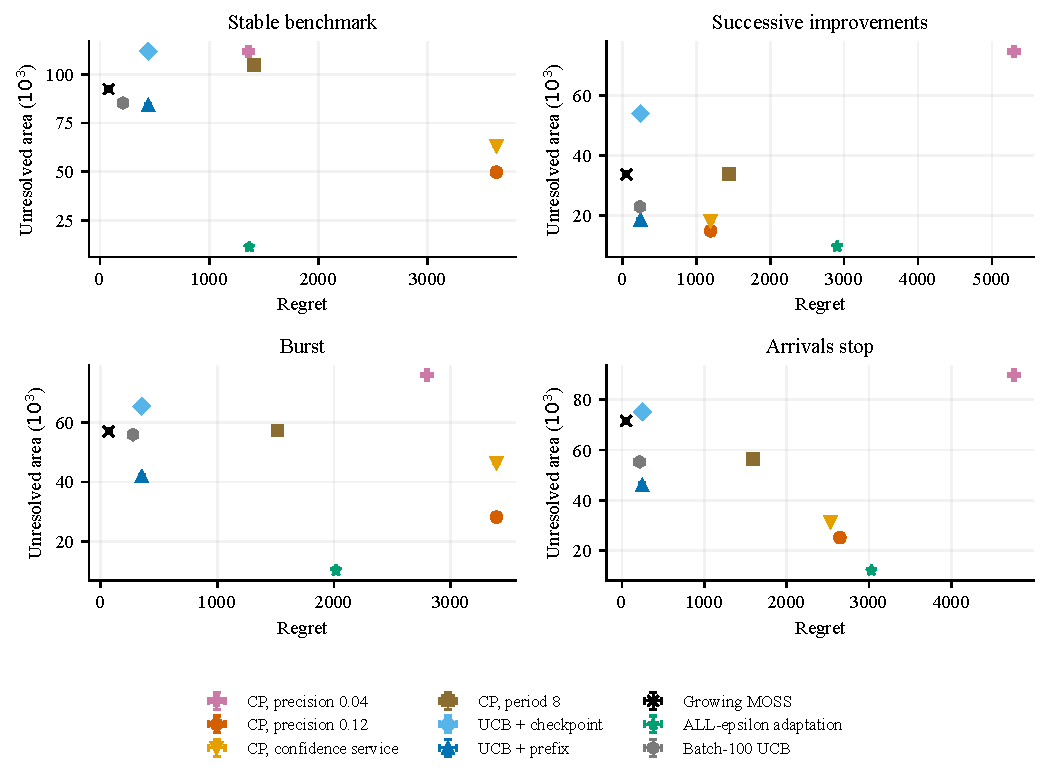
\includegraphics[width=.97\textwidth]{figures/fig_cost_area.pdf}
\caption{Regret and cumulative $\eta$-unresolved area for all nine methods.
Lower values on both axes are preferable. CP denotes the Checkpoint-UCB
configurations described in the text. Error bars quantify Monte Carlo
uncertainty. Neither checkpoint precision nor its allocation variants
uniformly dominate the confidence-based adaptation.}
\label{fig:cost-area}
\end{figure}

\subsection{Finite-budget findings and their limits}

In all 640 finer-checkpoint runs, every available arm remains unresolved
at every time step. Five to eight arms contribute to the final
$\eta$-unresolved count because the metric exempts the boundary band;
the remaining arms have not been classified. Its zero-error record
therefore does not establish useful classification at this budget.
The charged unresolved area ranges from 74,820 to 111,784. This is a
limitation of the conservative construction at the chosen budget.
The confidence-based adaptation resolves every $\eta$-separated arm by
the endpoint in all replications of these four environments.

The coarser checkpoints reduce area relative to UCB alone, but can incur
much larger regret. Under the stable benchmark, CP-FIFO has mean regret
3629.9 and area 49,718, compared with 1367.8 and 11,306 for
ALL-$\varepsilon$ adaptation. The paired differences, CP-FIFO minus the
adaptation, are $2262.1$ (standard error $11.7$) for regret and
$38{,}411.7$ (standard error $241.9$) for area. The adaptation improves
both quantities in the burst environment as well. These findings do not
support a general numerical advantage of checkpoint FIFO over a strong
history-retaining identification rule.

Under successive improvements, CP-FIFO occupies a different cost point:
regret 1194.7 and area 14,743, compared with 2905.8 and 9525 for the
adaptation. The paired regret difference is $-1711.0$ (standard error
$2.4$), and the area difference is $5217.7$ (standard error $141.1$).
This comparison does not isolate task expiration. The adaptation uses
all 10,000 designated service pulls, whereas coarse CP uses about 5,786;
some remaining questions fall inside the unpenalized boundary band.
The regret difference can therefore partly reflect different stopping
rules for reporting work. Identifying the mechanism requires a comparison
with the same boundary tolerance and service requirement. These observed
cost points do not estimate an optimal frontier.

Growing-MOSS has the smallest mean regret in all four environments,
between 52.0 and 77.3, while leaving substantially larger unresolved
areas. Small regret alone provides little evidence of timely set
maintenance; it does not rule out adding an effective certification
layer to that allocation rule. Explicit service pays for observations of
inferior arms. Reducing service from every second to every eighth pull
generally reduces regret and enlarges unresolved area. Confidence-driven
checkpoint service does not uniformly improve either criterion.

\begin{figure}[t]
\centering
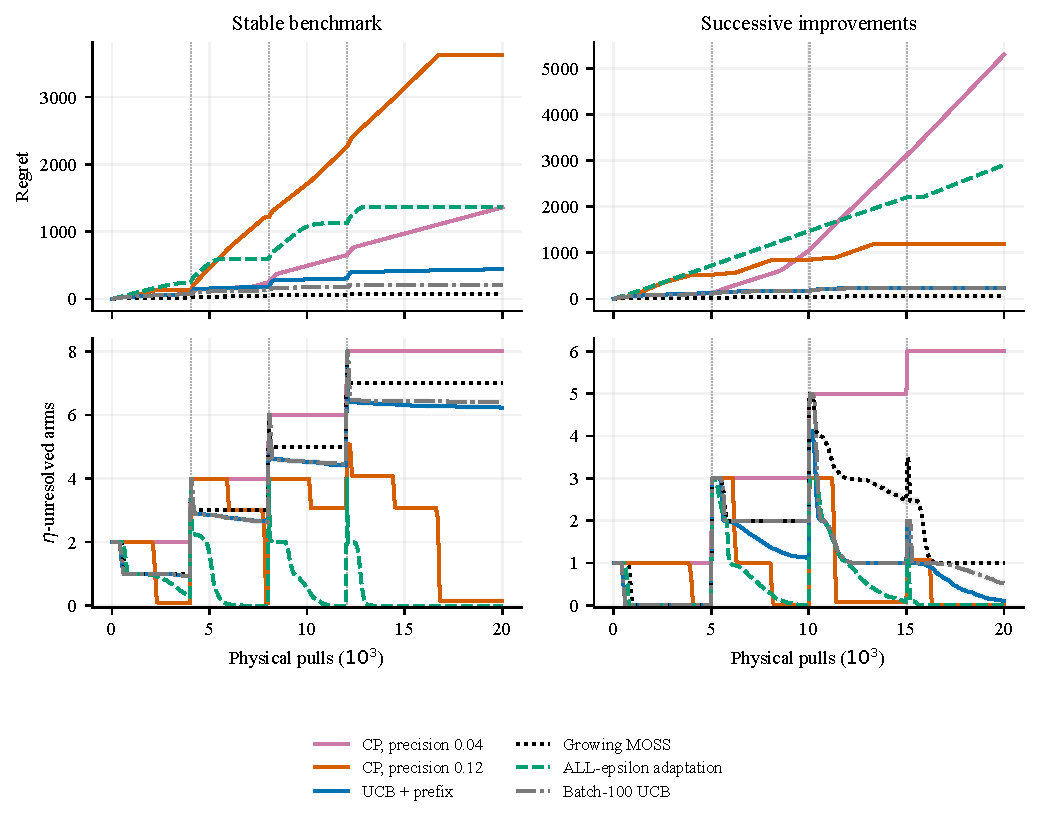
\includegraphics[width=.98\textwidth]{figures/fig_paths_pair1.pdf}
\caption{Mean regret and mean $\eta$-unresolved arm counts at the physical
sampling clock. Bands are 1.96 Monte Carlo standard errors; vertical dotted
lines mark arrivals. Stable and improving benchmarks are shown here,
with the other two environments in Appendix~\ref{app:computation}.
The six main-table methods are displayed. The saved results retain all
nine methods and their paths on the common observation grid.}
\label{fig:paths}
\end{figure}

For Batch100-UCB, the admission-delay contributions to regret are $0$,
$33.92$, $16.00$, and $22.40$ in the four environments. No historical
retirement deficit occurred in these runs. Appendix~\ref{app:computation}
defines this decomposition and distinguishes it from learning within the
reward-active set.

There were no incorrect positive or negative reports in any of the 5,760
runs. For one fixed method and environment, zero failures in 160
replications gives an exact one-sided 95\% upper confidence bound below
0.0186 on its failure probability. This finite experiment does not
establish uniform reliability over all environments and times. Nor do
the eight-arm comparisons validate the asymptotic lower bounds, settle
the critical logarithmic gap, or establish checkpoint optimality.
They quantify the finite-budget cost of the conservative quotas and
show why reward and maintenance must be reported together.

\section{Discussion}
\label{sec:discussion}

Reliable maintenance has costs that reward allocation alone does not
measure. An uncertain arrival can obstruct many positive reports, while
a later improvement can end an earlier fine classification task. The
common-reference lower bound and the repeated-update construction
isolate these effects. The matching worst-schedule area bound answers a
different question: its lower bound is already attained by a static
initial batch. The corresponding growth consequences depend on whether
the guarantee concerns one infinite schedule or a uniform terminal-count
class.

Checkpoint-UCB is an explicit attainability construction with a
predetermined reporting precision. It reuses accumulated evidence and
keeps all arrived arms eligible for rewards. Its upper bounds describe
achievable statistical costs, but do not imply competitive constants at
moderate budgets. In the numerical study the finer checkpoints never
produced a determinate label, and the coarser configuration was worse
than the retained-history identification adaptation in both displayed
costs in two environments. Practical comparisons must therefore match
the reporting task and required service level, as well as reward cost.

On the specified repeated-update family, rapid maintenance has matching
expected-regret and joint-quantile orders. The deferred endpoint supplies
an upper bound at a larger area budget. A matching deferred converse,
the frontier at intermediate budgets, and achievable guarantees under
general overlapping arrivals remain unresolved. Automatic precision
selection also needs a valid confidence construction; choosing a
favorable checkpoint after inspecting its observations is outside the
fixed-precision guarantee. Mechanism experiments that separate evidence
reuse from service intensity and boundary-band work would help explain
finite-budget performance.

The supplement gives compatible-window truncations and a general
information-allocation relaxation as necessary conditions, together with
intermediate service configurations. It also proves eventual exact
classification for a separate revisable, multiresolution procedure when
arrivals stop, the final arm set is finite, and no arm lies on the
membership boundary. That consistency statement has different
assumptions and does not apply to fixed checkpoints. Contextual
information, delayed observations, and changing reward laws would require
further analysis.

\section*{Data and code availability}
The accompanying project contains the simulation configuration, 5,760
run-level records, shared-stream construction, implementation, and
plotting code used in this article. The configuration and recorded source
hashes identify the experiment versions; computational details are given
in the supplement. These are simulated data. A public repository or
permanent archive URL has not been specified in this manuscript.

\bibliographystyle{plainnat}
\bibliography{references}
\end{document}
